\documentclass[]{article}
\usepackage{graphicx}
\usepackage{wrapfig}
\usepackage{caption}
\usepackage{dirtree}
\usepackage{textpos}


\usepackage[T1]{fontenc}
\usepackage[utf8x]{inputenc}
\usepackage[english]{babel}
\usepackage{tikz-uml}


\usepackage{hyperref}
\hypersetup{colorlinks=true}

%fancy headers
\usepackage{fancyhdr}
\pagestyle{fancy}
\fancyhf{}
\lhead{Modern Internet Forum Software}
\rhead{\thepage}
\usepackage{lipsum}


\title{Modern Internet Forum Software \\ Project Proposal}
\author{James Oswald, Kyle Plummer, Kyler Randall, \\ Ethan Seligman, Ed Tomlinson, Nicholas Tymeson, Paing Htet}
\date{}

\begin{document}

\maketitle
\thispagestyle{fancy}

\section{Introduction}
\subsection{Background Knowledge}

\begin{wraptable}{r}{5.5cm}
\begin{tabular}{|l|l|}

\hline
\textbf{Software Name} & \textbf{Language} \\
\hline
bbPress & PHP \\
Beehive Forum & PHP \\
Discourse & Ruby, JavaScript \\
Discuz & PHP \\
FluxBB & PHP \\
FUDforum & PHP \\
Ikonboard & Perl \\
Invision Power Board & PHP \\
MyBB & PHP \\
Phorum & PHP \\
phpBB & PHP \\
PunBB & PHP \\
Syndie & Java \\
Thredded & Ruby \\
Vanilla Forums & PHP \\
vBulletin & PHP \\
\hline
\end{tabular}
\captionsetup{belowskip=0pt}
\caption{A list of top forum software and their back end languages. Note the dominance of PHP}
\end{wraptable}
\subsubsection{History}
\paragraph{}
Internet forums dominated the web as the primary method of online communication before the age of social media. Today, major social media platforms such as \href{https://www.reddit.com/}{reddit}, \href{https://www.4channel.org/}{4chan}, and others still use the forum model as the basis for interaction on their sites. Beyond these juggernauts, forums are still one of the most popular platforms for the online discussion of niche subjects and can be hosted by anyone with a passion and a web server. 
\paragraph{}
Forum software is the collection of client and server applications that handle the running and data flow of a forum. The golden age of forums coincided with the height of popularity of PHP and the LAMP stack. Therefore it should be no surprise that PHP dominates the landscape of internet forum software. 
\subsubsection{The Modern Ecosystem}
\paragraph{}
Unfortunately most of these PHP forum applications, while still well maintained, lack the ability to keep up in today's modern web software ecosystems. 
\begin{textblock}{5}(5, -7)
For a table of contents, \hyperref[cont]{Click Here}.
\end{textblock}

\paragraph{}
Modern web software is built in a more modular manner. This software makes use of design patterns like MVC to handle all interface processing client side using technologies like React and Angular. The aforementioned legacy form software instead used PHP to preform rendering (hypertext pre-processing) of the page server side, which was costly and inefficient. In addition web developers just aren't as interested in PHP as a language anymore. Developers are moving to newer server side technology like Node.js and Express to replace PHP back ends, and MongoDB to replace SQL. 

\subsection{Project Significance}
\paragraph{}
The goal of this project is to develop an Internet Forum Software package using a modern stack that can act as a lightweight replacement to the legacy PHP forum software written for the LAMP stack. A modern forum project has wide reaching applications for website customers looking to host forums on their sites. Many customers desire a forum but quickly learn that all the best forums are PHP based. This can force customers to use older PHP software, which isn't as friendly to cloud computing and other accelerating technologies that are geared towards modern stacks. By developing this software, you will provide customers a drop in replacement for legacy systems, and a new paradigm for their website that will bring time tested forum technology into the modern era. 

\section{Structure and Function Background}
\paragraph{}
Before getting into requirements it is essential that one understands the structures and functions of internet forums. Please note, while these are not the requirements, your forum must conform to these basic archetypes, as the requirements proceed assuming these are a given. 

\subsection{General Site Structure Overview}\label{structOver}
\begin{minipage}{0.65\textwidth}
\paragraph{}
All forums follow a basic structural pattern of a four level hierarchy (Referred form here on out as 4LH): Home $\to$ Topic $\to$ Thread $\to$ Post. This compartmentalizes forums by breaking them into different sections each with higher specificity of discussion than the last. \ref{home} - \ref{post} provide a broad overview of the purposes of each of these sections.
\end{minipage}%
\hspace{0.5cm}
\vline
\hspace{0.5cm}
\begin{minipage}{0.35\textwidth}
\dirtree{%
.1 Home. 
.2 Topic. 
.3 Thread. 
.4 Post. 
}
\vspace{0.5 cm}
The 4 level hierarchy (4LH) pattern all forums follow.  
\end{minipage}%

\newpage

\subsubsection{Examples}\label{StructEx}
\paragraph{}
Throughout the explanation of the structure we will refer to three different popular forums (reddit, 4chan, MAL) as examples of different design decisions regarding the sections of the 4LH pattern. Each of these forums uses a 4LH, but they refer to its sections as different things and stylize them in different ways. To illustrate the 4LH sections the trees below provide a side by side comparison with hyperlinks to a sample of each section, and each depict how a forum refers to its sections. Please note that that each section is directly equivalent to the it's level on the 4LH ladder. Some forums' user terminology for one section is the same another forum uses for a different section. For example, MAL refers to it's threads as topics and reddit refers to it's threads as posts.
\paragraph{}

\begin{minipage}{0.3\textwidth}
\hspace{0.3cm}
\href{https://www.reddit.com/}{reddit}
\vspace{0.2 cm}
\dirtree{%
.1 \href{https://www.reddit.com/}{Homepage}. 
.2 \href{https://www.reddit.com/r/computerscience/}{Community}. 
.3 \href{https://www.reddit.com/r/computerscience/comments/igpuuf/computer_science_is_not_just_programming/}{Post}. 
.4 \href{https://www.reddit.com/r/computerscience/comments/igpuuf/computer_science_is_not_just_programming/g2vbikj?utm_source=share&utm_medium=web2x&context=3}{Reply}. 
}
\end{minipage}%
\vline
\begin{minipage}{0.3\textwidth}
\hspace{0.3cm}
\href{https://www.4channel.org/}{4chan}\footnotemark
\vspace{0.2 cm}
\dirtree{%
.1 \href{https://www.4channel.org/}{Home}. 
.2 \href{https://boards.4channel.org/g/}{Board}. 
.3 Thread. 
.4 Reply. 
}
\end{minipage}%
\footnotetext{Due to the nature of 4chan deleting threads after a few days, I cannot provide an active link to a thread or post, but feel free to look at them.}
\vline
\begin{minipage}{0.3\textwidth}
\hspace{0.3cm}
\href{https://myanimelist.net/}{MAL}\footnotemark
\vspace{0.2 cm}
\dirtree{%
.1 \href{https://myanimelist.net/forum/}{Home}. 
.2 \href{https://myanimelist.net/forum/?board=7}{Board}. 
.3 \href{https://myanimelist.net/forum/?topicid=1857368}{Topic}. 
.4 \href{}{Post}. 
}
\end{minipage}%
\footnotetext{Cannot link directly to posts on MAL}

\subsubsection{Home}\label{home}
\paragraph{}
The Home (AKA: Homepage) is the landing page for the forum as well as the primary navigation page for users to pick a topic they are interested in discussing. It contains the name of the forum as well as any branding the forum has (logos and motto's etc). It can highlight popular threads from all topics.

\paragraph{}
For example; reddit is a forum who's home features top threads, but doesn't have navigation to topics due to the millions of user created reddit communities. Other forums like 4chan and MAL only allow topics to be created by admins, so there is a set navigation layout on the homepage. On these homepages topics are often grouped on into categories. 

\subsubsection{Topic}
\paragraph{}
Topics (AKA: boards or communities) are containers for threads. A topic contains threads that are all about similar content (I.E. a forum about animals might have a dog topic, containing threads related to dogs). A topic will have its own page in which threads in that topic will be displayed, and the option to create new threads exists. How much about each thread is displayed varies by platform.
\paragraph{}
For example, reddit will display all threads ever posted, but only display the title and image. This allows users to vote on threads using the topic page. 4chan takes a different approach. It displays the fifteen most recently replied to threads and puts them on a page, and has 10 pages of threads per topic. 4chan opts to display the 5 most recent posts in the thread under the thread heading which contains a character capped preview of all the text in the opening thread post. MAL, a more traditional forum, displays the most recently replied to threads, but only display the name of the topic, when and who it was posted by, and when and who posted the last reply. 

\subsubsection{Thread}
\paragraph{}
A thread is a container for posts. Threads are the highest level structure that a normal user of a forum can create. A thread is started from a topic's page, and a post is the actual content of the message used to create the thread. A thread will have its own page for users to reply to the thread and each other.
\paragraph{}
For example, a reddit thread page lets users see all of the replies to a post and the replies to those replies (Please note that you don't need to implement a reddit like reply system). It also allows users to upvote and downvote replies. A 4chan thread has no direct reply system rather, 4chan allows posts to be "mentioned" by its post ID. In turn a MAL thread has a "quote" option under every post that will allow you to reply and allow other users to track your discussion by posting a minimized version of the quote chain above posts.    

\subsubsection{Post}\label{post}
\paragraph{}
A post is the smallest unit of discussion on a forum. A post is a message within a thread. A post will always contain text but may also allow an attached image, file, embed, or video. Users can reply to posts by creating their own posts, usually this will be done on the thread page and there will be no such thing as a "Post page" however some forums like reddit allow for an individual post in a thread to be linked too. 
\paragraph{}
reddit is an example of a forum that lets you upload multiple pieces of media when making a post but only if your post is the start of a thread. 4chan on the other hand allows only images but will allow one image to  be attached per post. MAL will allow both unlimited images and links in the initial and reply posts.

\subsection{User Structure}\label{usrStruct}
Any entity that makes threads, posts, manages, or even looks at the forum is a "User". Forum users vary significantly by desired forum model. Users will have "ranks" or "roles" that grant them certain elevated privileges and forum management options, or users may be anonymous guests and not have any account associated with them at all. 

\begin{minipage}{0.65\textwidth}
\paragraph{}
Much like site structure, most forums follow a structural hierarchy for users as well. This pattern is normally something along the lines of Admin $\to$ Moderator $\to$ User $\to$ Guest. This structure is top down, and allows for heightened content quality control by a sites administration.
\end{minipage}%
\hspace{0.5cm}
\vline
\hspace{0.5cm}
\begin{minipage}{0.35\textwidth}
\dirtree{%
.1 Administrator. 
.2 Moderator. 
.3 User. 
.4 Guest/Anon. 
}
\vspace{0.5 cm}
The forum user hierarchy (FUH)  
\end{minipage}%

\paragraph{}
Note that what we will now refer to as a "User" is a user with normal site permissions and not the abstract notion of a user that we have been discussing which by definition encompasses all four of these. It should also be noted that while roles follow the FUH, the true inheritance relationship between admins moderators and users is one of inheritance where admins and moderators are users, while guests are not.
\\\\\\
\textbf{UML Model of the FUH:} Associations (small arrows) represent ability to moderate, inheritance relations (white tipped arrows) represent Is-A relationships.
\vspace{0.5 cm}
\begin{center}
    \begin{tikzpicture} 
        \begin{umlpackage}[x=0, y=0]{Abstract User}
            \begin{umlpackage}[x=0, y=0]{Account User}
                \umlsimpleclass[x=1,y=-2]{Admin}
                \umlsimpleclass[x=1, y=0]{User}
                \umlsimpleclass[x=0,y=-4]{Moderator}
            \end{umlpackage}
            \umlsimpleclass[x=4,y=-2]{Guest}
        \end{umlpackage}
        %\umlinherit[anchor1=110, anchor2=-110]{Admin}{User}
        %\umluniassoc[anchor1=70, anchor2=-70]{Admin}{User}
        \umlinherit[geometry=|-, anchor1=160, anchor2=173]{Moderator}{User}
        \umluniassoc[geometry=|-, anchor1=150, anchor2=187]{Moderator}{User}
        \umluniassoc[geometry=-|, anchor1=-10, anchor2=-90]{Moderator}{Guest}
        \umluniassoc[geometry=--, anchor1=0, anchor2=180]{Admin}{Guest}
        \umluniassoc[geometry=--, anchor1=90, anchor2=-90]{Admin}{User}
        \umlinherit[geometry=--, anchor1=-147.5, anchor2=40]{Admin}{Moderator}
        \umluniassoc[geometry=--, anchor1=-137.5, anchor2=30]{Admin}{Moderator}
    \end{tikzpicture}
\end{center}

\newpage
\subsubsection{Examples}
Using the same three sites from \ref{StructEx}, we will analyze their user hierarchy in detail. and compare and contrast them in the following sections.

\vspace{0.2 cm}
\begin{minipage}{0.4\textwidth}
\hspace{0.3cm}
\href{https://www.reddit.com/}{reddit}
\vspace{0.2 cm}
\dirtree{%
.1 Reddit Admin. 
.2 Community Moderator. 
.3 User. 
.4 N/A\footnotemark. 
}
\end{minipage}%
\footnotetext{reddit does not allow posts by guests, must have an account.}
\vline
\begin{minipage}{0.23\textwidth}
\hspace{0.3cm}
\href{https://www.4channel.org/}{4chan}
\vspace{0.2 cm}
\dirtree{%
.1 Admin. 
.2 Mod.
.3 N/A\footnotemark.
.4 Anon. 
}
\end{minipage}%
\footnotetext{4chan has no accounts for normal users, rather everyone is a "Guest".\footnotemark[6]}
\vline
\begin{minipage}{0.4\textwidth}
\hspace{0.3cm}
\href{https://myanimelist.net/}{MAL}
\vspace{0.2 cm}
\dirtree{%
.1 Forum Administrator. 
.2 Forum Moderator. 
.3 User. 
.4 N/A\footnotemark.
}
\end{minipage}%
\footnotetext{MAL does not allow posts by guests, must have an account.}

\subsubsection{Administrators}
Administrators own the forum and have full access to all features including moderation, promotion, style, topic creation, etc. They are the only ones who can moderate moderators and each other. To create a forum, at least one admin account is necessary so that the forum can be managed after its creation. Most forums will display an admin badge or give admins a special name color when an Admin makes a post to let users know to pay extra-close attention to what is being said.    

\subsubsection{Moderators}
Moderators are generally the policemen of a forum. They have low level moderation work outsourced to them by administrators which is accomplished by patrolling and looking over flagged or reported posts. Moderators may also have elevated permissions to pin threads or create new topics depending on the forums settings.

\subsubsection{Users}
Users are the normal account holding users of a forum. It is safe to assume that on a regular forum, 99.9\% of abstract users will just be this level of regular user. In order to become a user, a forum will fist have you create an account, and then have you log in to use the forum. 

\subsubsection{Guests / Anons}
Anyone without an account is a "Guest". Guests usually can't post on normal forums and may not even be allowed to veiw any content. However, some forums like 4chan are almost exclusively used by accounts-less anonymous users, where only mods and admins have accounts.\footnotemark
\footnotetext{Anyone who really knows 4chan knows that this is a drastic simplification of the account system and that between pass users, tripcode users, and janitors there is more complexity then what could fit into this model.} 

\subsection{Security}
\paragraph{}
So that a forum can be more then just a proof of concept, every good forum needs security features. A wide range of forum security features exist across many of our example site, however since our security requirements will primarily be API driven using simple hashing, we will leave the examples to be researched independently. 

\section{Requirements}
\subsection{Goal}
\paragraph{}
Your task is to create a highly customizable forum software with a modern stack that provides forum administrators and users a fine degree of control over the style and features. 


\subsection{User Features}
\subsubsection{Forum User Hierarchy Features}
\paragraph{}
Your forum should follow the FUH provided in section \ref{usrStruct} and have moderation follow the moderation ability diagram from the UML in the same section. the have four user levels with configurable permissions.
\begin{enumerate}
    \item \textbf{Administrator (admin):} Top level accounts with full moderation, setting, and promotion access.
    \item \textbf{Moderator (mod):} Accounts with access to topic specific moderation. (Also referred to as topic moderators)
    \item \textbf{User:} Account with basic permissions to post.
    \item \textbf{Guest:} Users without an account who may or may not be able to post based on settings. 
\end{enumerate}

\subsubsection{User Creation Features}\label{UCF}
\begin{itemize}
    \item check for taken Username
    \item Email verification on account setup
    \item Password strength check
    \item Retype password check 
\end{itemize}

\subsubsection{User Customization Features}
These features hinge on weather or not they are enabled at setup, see \ref{setup}:\ref{custom}
\begin{itemize}
    \item \textbf{Profile Picture:} to display on threads, posts, and profile.
    \item \textbf{Nickname:} to replace their username as their display name after it has been set
    \item \textbf{Biography:} to be displayed on their profiles.
\end{itemize}

\subsubsection{Moderation and Promotion Features}
\begin{itemize}
    \item Ability for admins and topic mods to ban or mute a user from a topic.
    \item Ability for admins to ban or mute a user from the whole forum.
    \item Ability for admins to create moderators and other admins.
\end{itemize}

\subsection{Modes}
Your forum should have three modes that allow different states of operation. 
\begin{enumerate}
    \item \textbf{Setup:} One time setting of critical options that determine forum database layout.
    \item \textbf{Live:} Normal operation mode. 
    \item \textbf{Down:} Lets admins change setting and doesn't let normal users on until switched off.
\end{enumerate}

\subsection{Page Features}
Your forum site should follow the general layout of the 4LH model discussed in section \ref{structOver}. This means you should first be sure to implement the following pages.
\subsubsection{List of Pages to be Implemented}\label{Pages to implement}
\begin{enumerate}
    \item \textbf{Home Page:} List of boards / topics & options to create new boards.
    \item \textbf{Topic Pages:} Lists of threads on a topic & options to create new threads.
    \item \textbf{Thread Pages:} Lists of posts in a given thread
\end{enumerate}
On top of these provided by the 4LH model, you should also implement these standard auxiliary pages:
\begin{enumerate}
    \item \textbf{Setup Page:} Page for initial setup of the site in setup mode.
    \item \textbf{Down Page:} Page to display message notifying users the site is down.
    \item \textbf{Account Creation Page:} Page to create new user accounts.
    \item \textbf{Login Page:} Page to log into your account.
    \item \textbf{Profile Pages:} Pages for users with accounts to display information on themselves.
    \item \textbf{User settings Pages:} Pages for users with accounts can change their settings.
    \item \textbf{Rules Pages:} For the rules of the forum or sub-rules for certain topics. 
    \item \textbf{404 Page:} For 404 (Page not found) errors. 
    \item \textbf{500 Page:} For 500 (Internal Server) errors.
\end{enumerate}

\subsubsection{Universal Page Features}\label{uni}
The following features should be present on every single page.
\begin{itemize}
    \item The forum's header, with links to key parts of the forum, the name, and the logo.
    \item A user button with user navigation links to their profile and settings.
    \item A modular HTML Class and ID system that can easily be customized using user uploaded CSS style sheets.
\end{itemize}

\subsubsection{Setup Page Features}\label{setup}
The setup page should include the following features:
\begin{enumerate}
    \item \label{anon} A config option allowing or disallowing guests to post Under Nicknames or Anonymously.
    \item \label{votes} Three config options allowing or disallowing voting on Topics, Threads, and Posts.
    \item \label{modgod} A config option allowing or disallowing users to have the ability create and moderate their own topics (Boards / Communities).
    \item A config option specifying how long or how many inactive threads to store, or weather or not to delete them at all. 
    \item \label{custom} Three config options allowing or disallowing users to have profile pictures, signatures, and nicknames.
    \item \label{pfp} A config options allowing or disallowing profile pages.
    \item \label{attachments} Configuration options on what type of files are allowed to be attached to posts.
\end{enumerate}

\subsubsection{Home Page Features}
The home page should have the following features:
\begin{itemize}
    \item Ability for admins (potentially moderators, see \ref{setup}:\ref{modgod}) to create and delete topics
    \item A sort-able and search-able list of all topics based on activity, posts, popularity, time, or potentially votes (see \ref{setup}:\ref{votes}) 
    \item Featured threads pulled from all topics based on activity, posts, popularity, time, or potentially votes (see \ref{setup}:\ref{votes}) 
\end{itemize}

\subsubsection{Topic Pages Features}
\begin{itemize}
    \item Ability for users (potentially guests, see \ref{setup}:\ref{anon}) to create new threads or delete threads that they've made.
    \item A sort-able and search-able list of all threads based on activity, posts, popularity, time, or potentially votes (see \ref{setup}:\ref{votes}) 
    \item Ability for admins and mods to delete threads from the topic page.
\end{itemize}

\subsubsection{Thread Pages Features}\label{threadF}
\begin{itemize}
    \item Ability for users (potentially guests, see \ref{setup}:\ref{anon}) to create new posts or edit and delete posts that they've made.
    \item Ability for admins and mods to delete posts.
    \item A sort-able and search-able list of all posts in the thread based on activity, posts, popularity, time, or potentially votes (see \ref{setup}:\ref{votes}) 
    \item Ability to sort posts by reply, using either a reply citation system like 4chan or a quote reply system like MAL, you do not need to implement a reply chain system like reddit.
\end{itemize}

\subsubsection{Post Features}
While not explicitly a page unto themselves, these features fit best here. 
\begin{itemize}
    \item Ability to send text data.
    \item Ability to be edited or deleted by the user who posted it.
    \item Ability to be deleted by admins or topic mods.
    \item Ability to attach certain media types such as images if the config from \ref{setup}:\ref{attachments} is set true.
    \item Ability for admins or topic mods to remove attachments without deleting the post. 
    \item Ability to reply to other posts using a quotation system or reply citation system as mentioned in \ref{threadF}
\end{itemize}

\subsubsection{Account Creation Page Features}
\begin{itemize}
    \item All of the features mentioned and inferred from in \ref{UCF}.
    \item A captcha to prevent botting account creation.
\end{itemize}

\subsubsection{Login Page Features}
\begin{itemize}
    \item A place to enter your username and password.
    \item A captcha to prevent botting account logins.
\end{itemize}

\subsubsection{User settings Pages Features}
\begin{itemize}
    \item Ability to change any enabled user settings, profile pic, nickname, bio, password, etc. Note that Username is not changeable!
    \item Ability to upload a custom CSS style-sheet to restyle the modular layout forum specified in section \ref{uni}.
\end{itemize}


\subsubsection{Profile Pages Features}
The existence of these hinges on \ref{setup}:\ref{pfp} being enabled.
\begin{itemize}
    \item Whichever of the items are enabled from \ref{setup}:\ref{custom}.
    \item Number of posts.
    \item Registration date.
\end{itemize}

\subsubsection{Article 10}
Any pages listed in \ref{Pages to implement} but not listed in any of the other subsections 3.5 subsections are to be implemented at your discretion, but still must follow the Universal Page Features from section \ref{uni}.

\newpage
\subsection{Security}
The forum must implement some standard security features so that its actually usable as more then just a proof of concept. 
\subsubsection{Data Storage Requirements}\label{dsr}
You must ensure a high level of data security as you will be storing account information.
\begin{itemize}
    \item No plain text stored in the database for anything. Especially user credentials. 
    \item Use a modern hashing method to ensure all encrypted data is cryptographically secure from being decoded if the data is stolen. 
\end{itemize}

\subsubsection{Spam Prevention Requirements} \label{spamprev}
Users should not be able to spam create threads or posts or anything that could potentially increase server load using a single account or guest IP.
\begin{itemize}
    \item A reasonable post and thread cool down time between post and thread creations for a single user.
    \item Auto-ban / auto-mute anyone clearly advertising or spamming the same message. For guest users this should be implemented as an IP ban.
    \item A reasonable attachment max size and attachment garbage collection to prevent intentionally running down disk space.
    \item Countermeasures for users spamming setting changes and trying to run down resources that way. 
\end{itemize}

\subsubsection{Bot Prevention Requirements}
You must protect against bots not only with the spam prevention requirements laid out in \ref{spamprev} but also brute forcing logons or account creation.
\begin{itemize}
    \item captacha on account creation, login, or when making multiple posts in a row. 
\end{itemize}

\subsubsection{Injection Prevention Requirements}
Users must not be allowed to inject code to run client or server side.
\begin{itemize}
    \item User input sanitation for ANYTHING sent to the server by users.
    \item Prevention of <script>s being put in posts or anything else the user inputs.
    \item Prevention of database query injection attacks that could leak user credentials. Even if this occurs, you should be double protected via the strict data storage requirements in section \ref{dsr}
\end{itemize}


\newpage
\section{Contents}\label{cont}
\tableofcontents
\vspace{8cm}
\begin{figure}[!h]
    \centering
    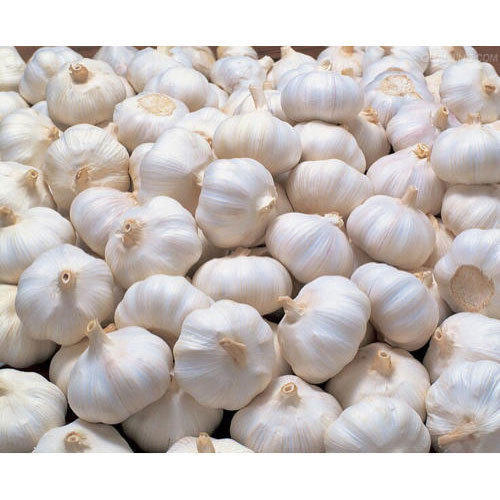
\includegraphics[scale=0.3]{Garlic.jpg}
    \caption{This project was brought to you by \href{https://github.com/UAlbany-Team-Garlic}{UAlbany Team Garlic}}
\end{figure}


\end{document}

